\documentclass[border=10pt]{standalone}

\usepackage{tikz}
\usepackage{tikzsymbols}
\usetikzlibrary{calc,patterns,shapes.geometric}

\def\centerarc[#1](#2)(#3:#4:#5){\draw[#1] ($(#2)+({#5*cos(#3)},{#5*sin(#3)})$) arc (#3:#4:#5);}

\begin{document}
	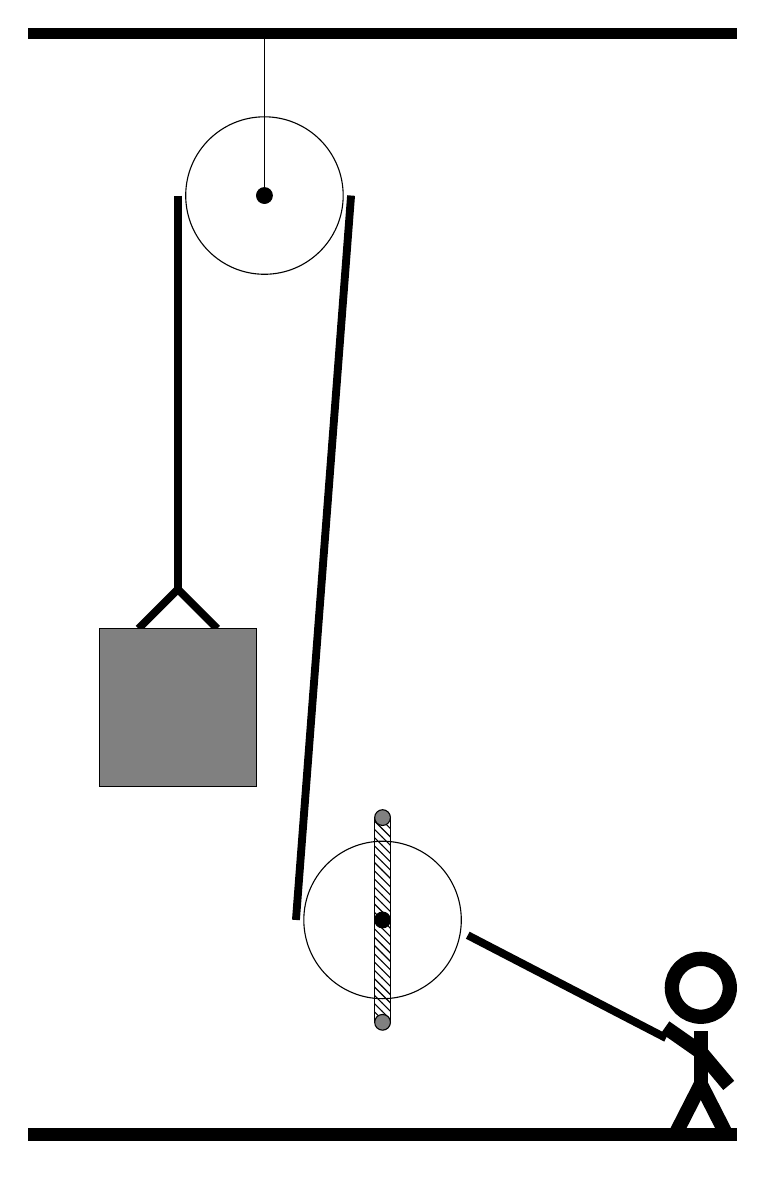
\begin{tikzpicture}
		%%%%% START %%%%%
		\draw[fill=black] (-2, 14) rectangle (7, 14.125);
		
		\draw (1, 12) circle (1);
		\draw[fill=black] (1, 12) circle (0.1);
		\draw (1, 14) -- (1, 12);
		
		\draw[fill=white](2.5, 2.8) circle (1);
		\draw[fill=black] (2.5, 2.8) circle (0.1);
		\draw[pattern=north west lines, pattern color=black] (2.4, 4.1) rectangle (2.6, 1.5);
		\draw[fill=black!50] (2.5, 4.1) circle (0.1);
		\draw[fill=black!50] (2.5, 1.5) circle (0.1);
		
		\draw[line width=1mm] (-0.6, 6.5) -- (-0.1, 7.0) -- (0.4, 6.5);
		\draw[fill=black!50] (-1.1, 6.5) rectangle (0.9, 4.5);
		
		\draw[line width=1mm] (-0.1, 12) -- (-0.1, 7.0);
		\centerarc[line width=1mm](1, 12)(0:180:1.1);
		\draw[line width=1mm](2.1, 12) -- (1.4, 2.8);
		\centerarc[line width=1mm](2.5, 2.8)(180:270:1.1);
		\draw[line width=1mm](3.582, 2.606) -- (6.1, 1.3);
		
		\node at (6.5, 1.2) {\Strichmaxerl[10][-35][-50]};
		
		\draw[fill=black] (-2, 0) rectangle (7, 0.15);
		%%%%% END %%%%%
	\end{tikzpicture}
\end{document}